% ------------------------------------------------------------------------------
% TYPO3 CMS 7.2 - What's New - Chapter "Introduction" (English Version)
%
% @author	Michael Schams <schams.net>
% @license	Creative Commons BY-NC-SA 3.0
% @link		http://typo3.org/download/release-notes/whats-new/
% @language	English
% ------------------------------------------------------------------------------
% LTXE-CHAPTER-UID:		16517900-07a67f43-fe9f3e35-7e924788
% LTXE-CHAPTER-NAME:	Introduction
% ------------------------------------------------------------------------------

\section{Introduction}
\begin{frame}[fragile]
	\frametitle{Introduction}

	\begin{center}\huge{Introduction}\end{center}
	\begin{center}\huge{\color{typo3darkgrey}\textbf{The Facts}}\end{center}

\end{frame}

% ------------------------------------------------------------------------------
% LTXE-SLIDE-START
% LTXE-SLIDE-UID:		8d8b89f9-f7c3da13-4412b0cd-af1d14f7
% LTXE-SLIDE-ORIGIN:	6d5e9f3e-f9d9677e-43d7d497-e80ba9ef English
% LTXE-SLIDE-TITLE:		TYPO3 CMS 7.2 - The Facts
% ------------------------------------------------------------------------------
\begin{frame}[fragile]
	\frametitle{Introduction}
	\framesubtitle{TYPO3 CMS 7.2 - The Facts}

	\begin{itemize}
		\item Release date: 28 April 2015
		\item Releasetyp: "Sprint Release"
		\item Vision: Embrace, Innovate, Deliver
		\item Primary focus: Frontend
	\end{itemize}

	\begin{figure}
		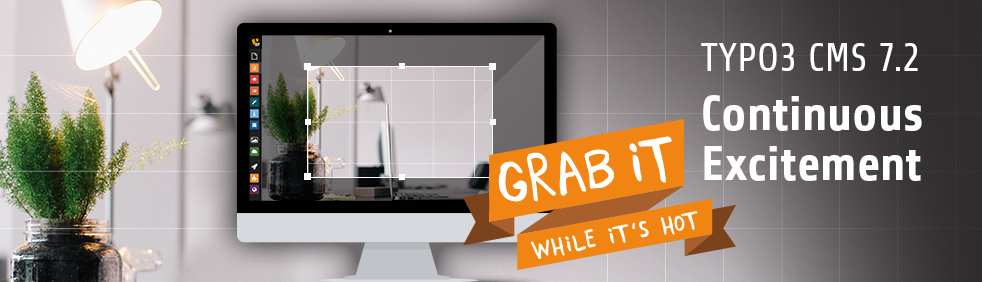
\includegraphics[width=0.95\linewidth]{Introduction/typo3cms72-teaser.png}
	\end{figure}

\end{frame}

% ------------------------------------------------------------------------------
% LTXE-SLIDE-START
% LTXE-SLIDE-UID:		967af102-2d3ba167-5fccfb15-fb5d2ef6
% LTXE-SLIDE-ORIGIN:	759c3860-d5061f6e-2bb0009f-6ea130c8 English
% LTXE-SLIDE-TITLE:		System Requirements
% ------------------------------------------------------------------------------
\begin{frame}[fragile]
	\frametitle{Introduction}
	\framesubtitle{System Requirements}

	\begin{itemize}
		\item PHP*:\tabto{2.2cm}v5.5.0 - v5.6.x
		\item MySQL:\tabto{2.2cm}v5.5.x - v5.6.x (no strict mode)
		\item Disk space:\tabto{2.2cm}min 200 MB
		\item PHP settings:

			\begin{itemize}
				\item memory\_limit >= 128M
				\item max\_execution\_time >= 240s
				\item compilation option \texttt{--disable-ipv6} must \underline{not} be used
			\end{itemize}

		\item Backend requires IE >= 9 or any other modern browser

	\end{itemize}

	\vspace{1cm}
	*) Further details: \href{http://typo3.org/news/article/php-minimum-requirements-for-typo3-cms-7/}{PHP Minimum Requirements for TYPO3 CMS 7}

\end{frame}

% ------------------------------------------------------------------------------
% LTXE-SLIDE-START
% LTXE-SLIDE-UID:		b89d9bba-4c0eacbf-d117ed3b-924b254c
% LTXE-SLIDE-ORIGIN:	70c77c41-e2b83d82-2f182996-98061070 English
% LTXE-SLIDE-TITLE:		Development And Release Timeline
% ------------------------------------------------------------------------------
\begin{frame}[fragile]
	\frametitle{Introduction}
	\framesubtitle{Development And Release Timeline}

	\begin{figure}
		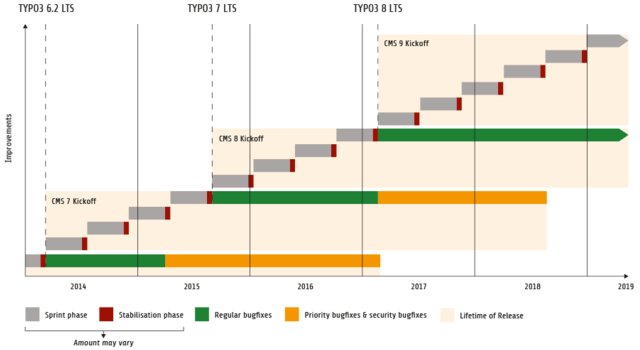
\includegraphics[width=0.90\linewidth]{Introduction/ReleaseAgenda.png}
	\end{figure}

\end{frame}

% ------------------------------------------------------------------------------
% LTXE-SLIDE-START
% LTXE-SLIDE-UID:		8a9b8ef6-0ec1bb74-fc63027a-9e8e8f27
% LTXE-SLIDE-ORIGIN:	b55d3fe9-76807061-d97f3fee-7db1f190 English
% LTXE-SLIDE-TITLE:		TYPO3 CMS Roadmap
% ------------------------------------------------------------------------------
\begin{frame}[fragile]
	\frametitle{Introduction}
	\framesubtitle{TYPO3 CMS Roadmap}

	Estimated release dates and their primary focus:

	\begin{itemize}
		\item v7.0 \tabto{1.0cm}02/Dec/2014\tabto{3.4cm}Backend Overhaul Vol 1
		\item v7.1 \tabto{1.0cm}24/Feb/2015\tabto{3.4cm}Core Cleanup \& Streamlining

		\item
			\begingroup
				\color{typo3orange}
					v7.2 \tabto{1.0cm}28/Apr/2015\tabto{3.4cm}Frontend
			\endgroup

		\item v7.3 \tabto{1.0cm}09/Jun/2015\tabto{3.4cm}Package Ecosystem, Composer\newline
			\tabto{3.4cm}and Extension Handling
		\item v7.4 \tabto{1.0cm}04/Aug/2015\tabto{3.4cm}Backend Overhaul Vol 2
		\item v7.5 \tabto{1.0cm}29/Sep/2015\tabto{3.4cm}\textit{(to be determined...)}
		\item v7.6 \tabto{1.0cm}xx/xxx/2015\tabto{3.4cm}\textbf{TYPO3 CMS 7 LTS} (Long Term Release)
	\end{itemize}

	\smaller
		\url{https://typo3.org/typo3-cms/roadmap/}\newline
		\url{http://typo3.org/news/article/embrace-and-innovate-typo3-cms-7/}
	\normalsize

\end{frame}

% ------------------------------------------------------------------------------
% LTXE-SLIDE-START
% LTXE-SLIDE-UID:		5d84eaa5-03083d82-4855b465-64a70a60
% LTXE-SLIDE-ORIGIN:	b0c28f26-c3ca2e99-195954a8-ed76f9d4 English
% LTXE-SLIDE-TITLE:		Installation
% ------------------------------------------------------------------------------
\begin{frame}[fragile]
	\frametitle{Introduction}
	\framesubtitle{Installation}

	\begin{itemize}
		\item Official installation procedure under Linux/Mac OS X\newline
			(DocumentRoot for example \texttt{/var/www/site/htdocs}):
		\begin{lstlisting}
			$ cd /var/www/site
			$ wget --content-disposition get.typo3.org/7.2
			$ tar xzf typo3_src-7.2.0.tar.gz
			$ cd htdocs
			$ ln -s ../typo3_src-7.2.0 typo3_src
			$ ln -s typo3_src/index.php
			$ ln -s typo3_src/typo3
			$ touch FIRST_INSTALL
		\end{lstlisting}

		\item Symbolic links under Microsoft Windows:

			\begin{itemize}
				\item Use \texttt{junction} under Windows XP/2000
				\item Use \texttt{mlink} under Windows Vista and Windows 7
			\end{itemize}

	\end{itemize}
\end{frame}

% ------------------------------------------------------------------------------
% LTXE-SLIDE-START
% LTXE-SLIDE-UID:		abb1e380-9e73b4b6-c8e11fba-d90827d5
% LTXE-SLIDE-ORIGIN:	48136734-ae508d23-bce5811d-667f8908 English
% LTXE-SLIDE-TITLE:		Upgrade to TYPO3 CMS 7
% ------------------------------------------------------------------------------
\begin{frame}[fragile]
	\frametitle{Introduction}
	\framesubtitle{Upgrade to TYPO3 CMS 7.x}

	\begin{itemize}
		\item Upgrades only possible from TYPO3 CMS 6.2 LTS
		\item TYPO3 CMS < 6.2 should be updated to TYPO3 CMS 6.2 LTS first
	\end{itemize}

	\begin{itemize}

		\item Upgrade instructions:\newline
			\smaller\url{http://wiki.typo3.org/Upgrade#Upgrading_to_7.2}\normalsize
		\item Official TYPO3 guide "TYPO3 Installation and Upgrading":
			\smaller\url{http://docs.typo3.org/typo3cms/InstallationGuide}\normalsize
		\item General approach:
			\begin{itemize}
				\item Check minimum system requirements \small(PHP, MySQL, etc.)
				\item Review \textbf{deprecation\_*.log} in old TYPO3 instance
				\item Update all extensions to the latest version
				\item Deploy new sources and run Install Tool \textrightarrow Upgrade Wizard
				\item Review startup module for backend users (optionally)
			\end{itemize}
	\end{itemize}

\end{frame}

% ------------------------------------------------------------------------------
